% This file was created with tikzplotlib v0.10.1.
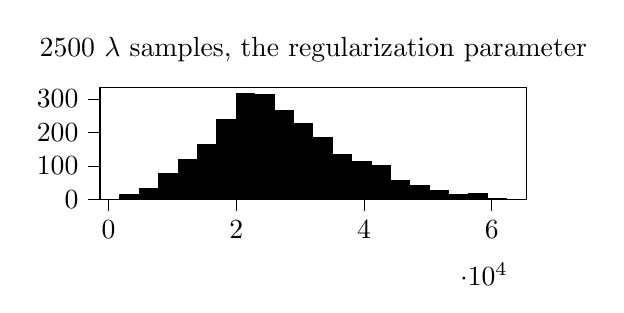
\begin{tikzpicture}

\definecolor{darkgray176}{RGB}{176,176,176}

\begin{axis}[
height=3cm,
tick align=outside,
tick pos=left,
title={2500 \(\displaystyle \lambda\) samples, the regularization parameter},
width=7cm,
x grid style={darkgray176},
xmin=-1323.66909320505, xmax=65472.0466137102,
xtick style={color=black},
y grid style={darkgray176},
ymin=0, ymax=332.85,
ytick style={color=black}
]
\draw[draw=none,fill=black] (axis cs:1712.49980256383,0) rectangle (axis cs:4748.6686983327,18);
\draw[draw=none,fill=black] (axis cs:4748.6686983327,0) rectangle (axis cs:7784.83759410158,34);
\draw[draw=none,fill=black] (axis cs:7784.83759410158,0) rectangle (axis cs:10821.0064898705,80);
\draw[draw=none,fill=black] (axis cs:10821.0064898705,0) rectangle (axis cs:13857.1753856393,122);
\draw[draw=none,fill=black] (axis cs:13857.1753856393,0) rectangle (axis cs:16893.3442814082,165);
\draw[draw=none,fill=black] (axis cs:16893.3442814082,0) rectangle (axis cs:19929.5131771771,239);
\draw[draw=none,fill=black] (axis cs:19929.5131771771,0) rectangle (axis cs:22965.682072946,317);
\draw[draw=none,fill=black] (axis cs:22965.682072946,0) rectangle (axis cs:26001.8509687148,314);
\draw[draw=none,fill=black] (axis cs:26001.8509687148,0) rectangle (axis cs:29038.0198644837,268);
\draw[draw=none,fill=black] (axis cs:29038.0198644837,0) rectangle (axis cs:32074.1887602526,229);
\draw[draw=none,fill=black] (axis cs:32074.1887602526,0) rectangle (axis cs:35110.3576560215,186);
\draw[draw=none,fill=black] (axis cs:35110.3576560215,0) rectangle (axis cs:38146.5265517903,135);
\draw[draw=none,fill=black] (axis cs:38146.5265517903,0) rectangle (axis cs:41182.6954475592,116);
\draw[draw=none,fill=black] (axis cs:41182.6954475592,0) rectangle (axis cs:44218.8643433281,103);
\draw[draw=none,fill=black] (axis cs:44218.8643433281,0) rectangle (axis cs:47255.033239097,59);
\draw[draw=none,fill=black] (axis cs:47255.033239097,0) rectangle (axis cs:50291.2021348659,42);
\draw[draw=none,fill=black] (axis cs:50291.2021348659,0) rectangle (axis cs:53327.3710306347,29);
\draw[draw=none,fill=black] (axis cs:53327.3710306347,0) rectangle (axis cs:56363.5399264036,17);
\draw[draw=none,fill=black] (axis cs:56363.5399264036,0) rectangle (axis cs:59399.7088221725,21);
\draw[draw=none,fill=black] (axis cs:59399.7088221725,0) rectangle (axis cs:62435.8777179414,6);
\end{axis}

\end{tikzpicture}
